\section{Case-1. Near-optimal layout}\label{case-1.-sub-optimal-layout}

In the first case \textbf{Access Points(APs)} are placed in the ground
so that both of them are in the center of the corresponding quarter of
25x25 meters and far from all UEs to approximately 25 meters.

\textbf{UEs} are left in two groups of three filling the other two
quarters respectively.

At the same time, they are not too close to each other in order to not
have interference and absolutely the same conditions.

Finally, \textbf{CnC} is set in the middle of the whole 50x50 meters an
experimental field, so that 2 APs and 2 groups of UEs mentioned above
are on the same distance.

This case expects to perform in the best signal quality and transmission
rate.

\begin{figure}[H]
	\centering
	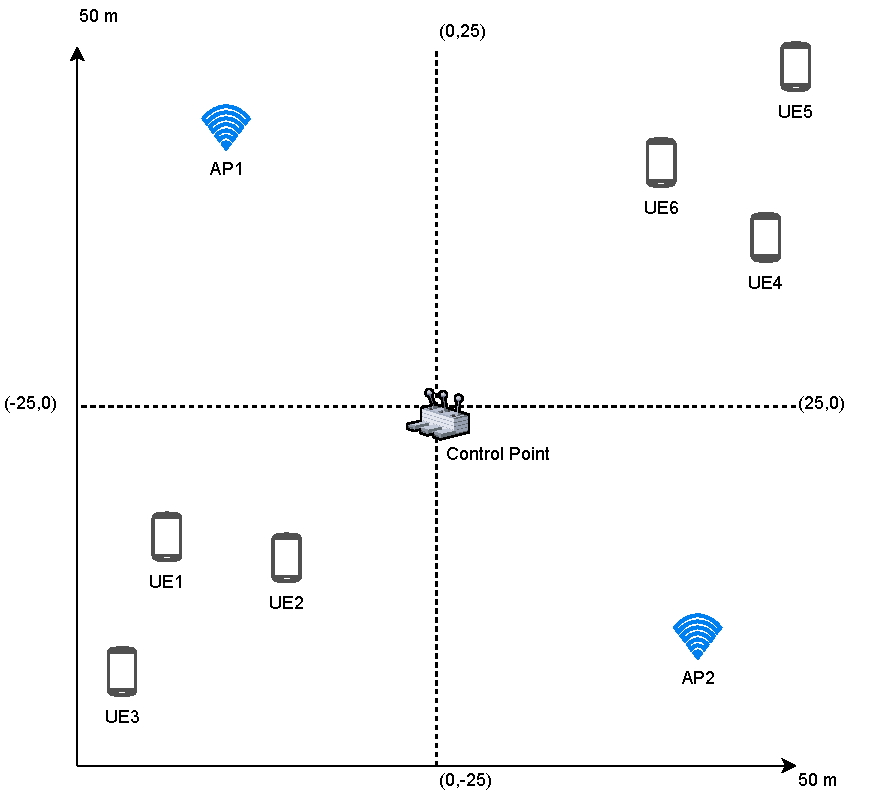
\includegraphics[width=\linewidth,keepaspectratio]{images/05-cases-description-Near-Optimal.pdf}
\caption{Near-optimal layout example}
\end{figure}
